\documentclass[final, hyperref={pdfpagelabels=false}]{beamer}
\usepackage[orientation=landscape,size=a0,scale=1.1]{beamerposter}
\usepackage[utf8]{inputenc}
\usepackage[T1]{fontenc}
\usepackage{helvet}
\renewcommand{\familydefault}{\sfdefault}

\usepackage{graphicx}
\usepackage{tikz}
\usetikzlibrary{shapes.geometric, arrows.meta, positioning, shadows}

% --- ULTIMATE CYBERPUNK NEON COLORS ---
\definecolor{bgdark}{RGB}{5, 10, 20}         % Deep space black
\definecolor{bgblock}{RGB}{15, 22, 38}        % Dark cyber panel
\definecolor{neoncyan}{RGB}{0, 243, 255}      % Glowing Cyan
\definecolor{neonmagenta}{RGB}{255, 0, 128}   % Glowing Magenta
\definecolor{neongreen}{RGB}{57, 255, 20}     % Hacker Green
\definecolor{techred}{RGB}{255, 0, 50}       % Alert Red
\definecolor{titletext}{RGB}{255, 255, 255}   % Pure white text
\definecolor{subtext}{RGB}{180, 200, 220}     % Muted icy blue text

% --- THEME & COLORS ---
\usetheme{boxes}
\setbeamercolor{background canvas}{bg=bgdark}
\setbeamercolor{headline}{bg=bgdark}
\setbeamercolor{title in headline}{fg=neoncyan}
\setbeamercolor{author in headline}{fg=titletext}
\setbeamercolor{institute in headline}{fg=subtext}

\setbeamercolor{block title}{fg=bgdark, bg=neoncyan}
\setbeamercolor{block body}{fg=titletext, bg=bgblock}
\setbeamercolor{item}{fg=neoncyan}

% --- HEADER SETUP ---
\setbeamertemplate{headline}{
  \leavevmode
  \begin{columns}
    \begin{column}{.1\paperwidth}
    \end{column}
    \begin{column}{.7\paperwidth}
      \vskip2cm
      \centering
      \usebeamercolor{title in headline}{\color{fg}\textbf{\fontsize{90}{110}\selectfont \inserttitle}\\[1ex]}
      \vskip1cm
      \usebeamercolor{author in headline}{\color{fg}\Large{\insertauthor}\\[1ex]}
      \usebeamercolor{institute in headline}{\color{fg}\large{\insertinstitute}\\[1ex]}
      \vskip1cm
    \end{column}
    \begin{column}{.2\paperwidth}
      \centering
      
\includegraphics[height=12cm]{logo.jpg}
    \end{column}
  \end{columns}
  \vskip2cm
}
\setbeamertemplate{footline}{}

% --- BLOCK STYLING ---
\setbeamertemplate{block begin}{
  \vskip.75ex
  \begin{beamercolorbox}[rounded=true,shadow=true,leftskip=1cm,colsep*=.75ex]{block title}%
    \usebeamerfont*{block title}\Large\textbf{\insertblocktitle}
  \end{beamercolorbox}%
  {\ifbeamercolorempty[bg]{block body}{}{\nointerlineskip\vskip-0.5pt}}%
  \usebeamerfont{block body}%
  \begin{beamercolorbox}[rounded=true,shadow=true,colsep*=.75ex,sep=1.5cm,vmode]{block body}%
    \ifbeamercolorempty[bg]{block body}{\vskip-.25ex}{\vskip-.75ex}\vbox{}%
}
\setbeamertemplate{block end}{
  \end{beamercolorbox}
  \vskip1cm 
}

% --- TIKZ FLOWCHART STYLES ---
\tikzset{
    process/.style={rectangle, draw=neoncyan, fill=bgdark, text=titletext, very thick, minimum width=8cm, minimum height=3cm, align=center, rounded corners, drop shadow},
    decision/.style={diamond, draw=neonmagenta, fill=bgdark, text=titletext, very thick, minimum width=4cm, minimum height=4cm, align=center, drop shadow},
    io/.style={trapezium, trapezium left angle=70, trapezium right angle=110, draw=neongreen, fill=bgdark, text=titletext, very thick, minimum width=8cm, minimum height=3cm, align=center, drop shadow},
    arrow/.style={-{Stealth[scale=1.5]}, neoncyan, thick, line width=2.5mm}
}

\title{NEURALFORENSICS: DEEP LEARNING FOR DEEPFAKE DETECTION}
\author{Prof. Dr. Shazzad Hosain \quad Dr. Md Adnan Arefeen \quad Nusaiba Al Mullick}
\institute{Dean of SEPS, NSU \quad $\mid$ \quad Assistant Professor, NSU \quad $\mid$ \quad NSU \\ North South University Cyber Security Center}

\begin{document}
\begin{frame}[fragile]
\begin{columns}[T]

% ==================== COLUMN 1 ====================
\begin{column}{.31\paperwidth}
\begin{block}{The Deepfake Threat}
    \vspace{1cm}
    \begin{center}
    \resizebox{0.9\linewidth}{!}{
        \begin{tikzpicture}[node distance=1.5cm and 2cm]
            \node (df) [circle, draw=neonmagenta, fill=bgblock, text=white, very thick, minimum size=5cm, align=center, drop shadow] {\Huge \textbf{DEEPFAKES}};
            \node (threat1) [rectangle, draw=neoncyan, fill=bgdark, text=white, very thick, minimum width=6cm, minimum height=2cm, align=center, above right=of df, xshift=1cm] {\LARGE \textbf{Misinformation}};
            \node (threat2) [rectangle, draw=neoncyan, fill=bgdark, text=white, very thick, minimum width=6cm, minimum height=2cm, align=center, right=of df, xshift=2cm] {\LARGE \textbf{Identity Theft}};
            \node (threat3) [rectangle, draw=neoncyan, fill=bgdark, text=white, very thick, minimum width=6cm, minimum height=2cm, align=center, below right=of df, xshift=1cm] {\LARGE \textbf{Erosion of Trust}};
            
            \draw [arrow, neonmagenta] (df) -- (threat1);
            \draw [arrow, neonmagenta] (df) -- (threat2);
            \draw [arrow, neonmagenta] (df) -- (threat3);
        \end{tikzpicture}
    }
    \end{center}
    \vspace{0.5cm}
\end{block}

\begin{block}{The Deep Learning Solution}
    \vspace{0.5cm}
    \begin{center}
    \resizebox{0.9\linewidth}{!}{
        \begin{tikzpicture}[node distance=1.5cm and 1cm]
            \node (cnn) [rectangle, draw=neongreen, fill=bgblock, text=white, very thick, minimum width=10cm, minimum height=3cm, align=center, drop shadow] {\Huge \textbf{Transformer-Based Model}};
            \node (adv1) [rectangle, draw=neoncyan, fill=bgdark, text=white, very thick, minimum width=5cm, minimum height=2cm, align=center, below left=1.5cm and -2cm of cnn] {\Large \textbf{Automated Detection}};
            \node (adv2) [rectangle, draw=neoncyan, fill=bgdark, text=white, very thick, minimum width=5cm, minimum height=2cm, align=center, below=2cm of cnn] {\Large \textbf{Sub-pixel Precision}};
            \node (adv3) [rectangle, draw=neoncyan, fill=bgdark, text=white, very thick, minimum width=5cm, minimum height=2cm, align=center, below right=1.5cm and -2cm of cnn] {\Large \textbf{100\% Local/Secure}};
            
            \draw [arrow, neongreen] (cnn) -- (adv1);
            \draw [arrow, neongreen] (cnn) -- (adv2);
            \draw [arrow, neongreen] (cnn) -- (adv3);
        \end{tikzpicture}
    }
    \end{center}
    \vspace{0.5cm}
\end{block}

\begin{block}{Neural Architecture}
    \vspace{1cm}
    \begin{center}
        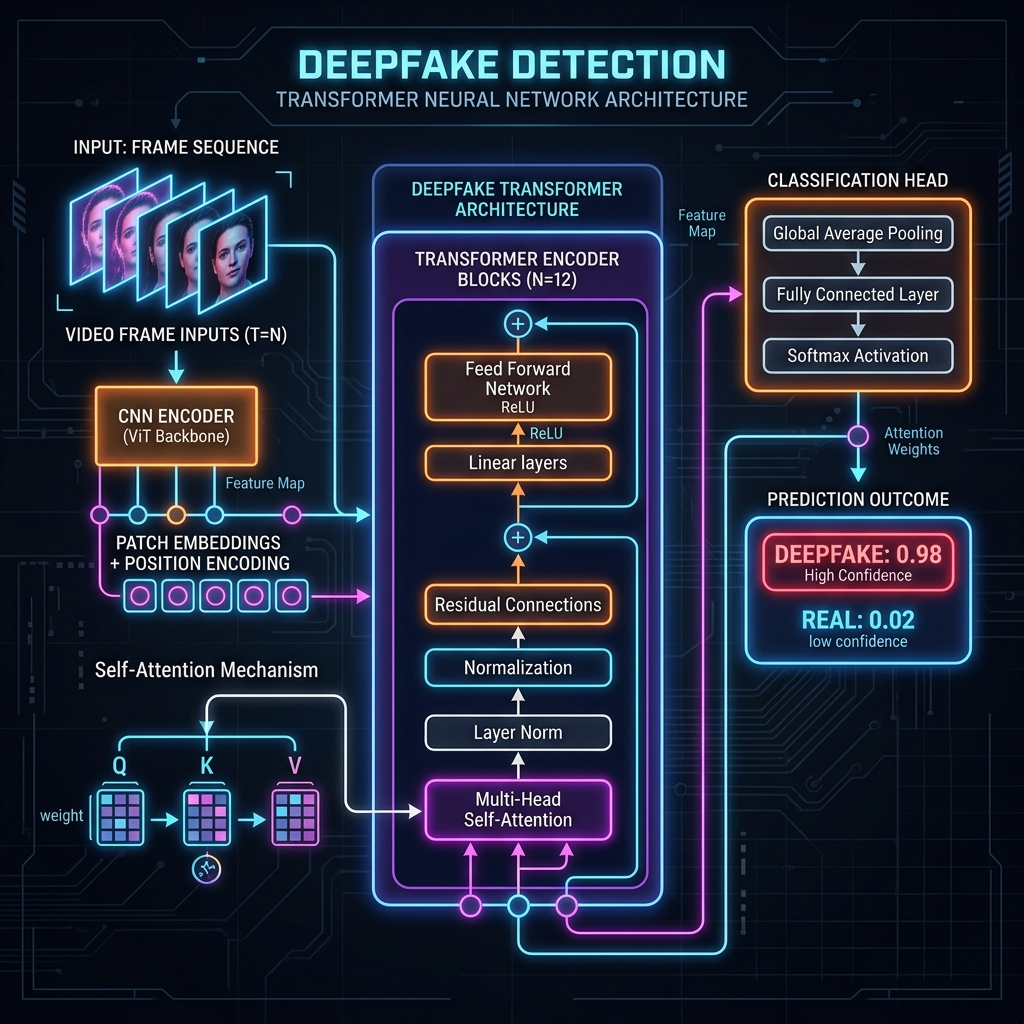
\includegraphics[width=0.9\linewidth]{sleek_diagram.jpg}
    \end{center}
    \vspace{0.5cm}
\end{block}
\end{column}

% ==================== COLUMN 2 ====================
\begin{column}{.31\paperwidth}
\begin{block}{AI Inference Pipeline}
    \vspace{1cm}
    \begin{center}
    \resizebox{0.95\linewidth}{!}{
        \begin{tikzpicture}[node distance=2.5cm and 2cm]
            \node (in) [io] {\textbf{Video Input} \\ (Raw Stream)};
            \node (sample) [process, below=of in] {\textbf{Frame Extraction} \\ (12 Distinct Frames)};
            \node (nn) [process, below=of sample] {\textbf{Transformer Model} \\ (Feature Extraction)};
            \node (agg) [process, below=of nn] {\textbf{Sigmoid Activation} \\ (Probability Score)};
            \node (dec) [decision, below=of agg] {\textbf{Mean} \\ $> 0.50$?};
            
            \node (fake) [io, right=of dec, draw=techred, text=techred, xshift=1cm] {\huge \textbf{SYNTHETIC}};
            \node (real) [io, left=of dec, draw=neongreen, text=neongreen, xshift=-1cm] {\huge \textbf{AUTHENTIC}};
            
            \draw [arrow] (in) -- (sample);
            \draw [arrow] (sample) -- (nn);
            \draw [arrow] (nn) -- (agg);
            \draw [arrow] (agg) -- (dec);
            \draw [arrow, techred] (dec) -- node[anchor=south, yshift=0.2cm, text=titletext] {\LARGE \textbf{Yes}} (fake);
            \draw [arrow, neongreen] (dec) -- node[anchor=south, yshift=0.2cm, text=titletext] {\LARGE \textbf{No}} (real);
        \end{tikzpicture}
    }
    \end{center}
    \vspace{1cm}
\end{block}

\begin{block}{Real-Time Artifact Localization}
    \vspace{1cm}
    \begin{center}
        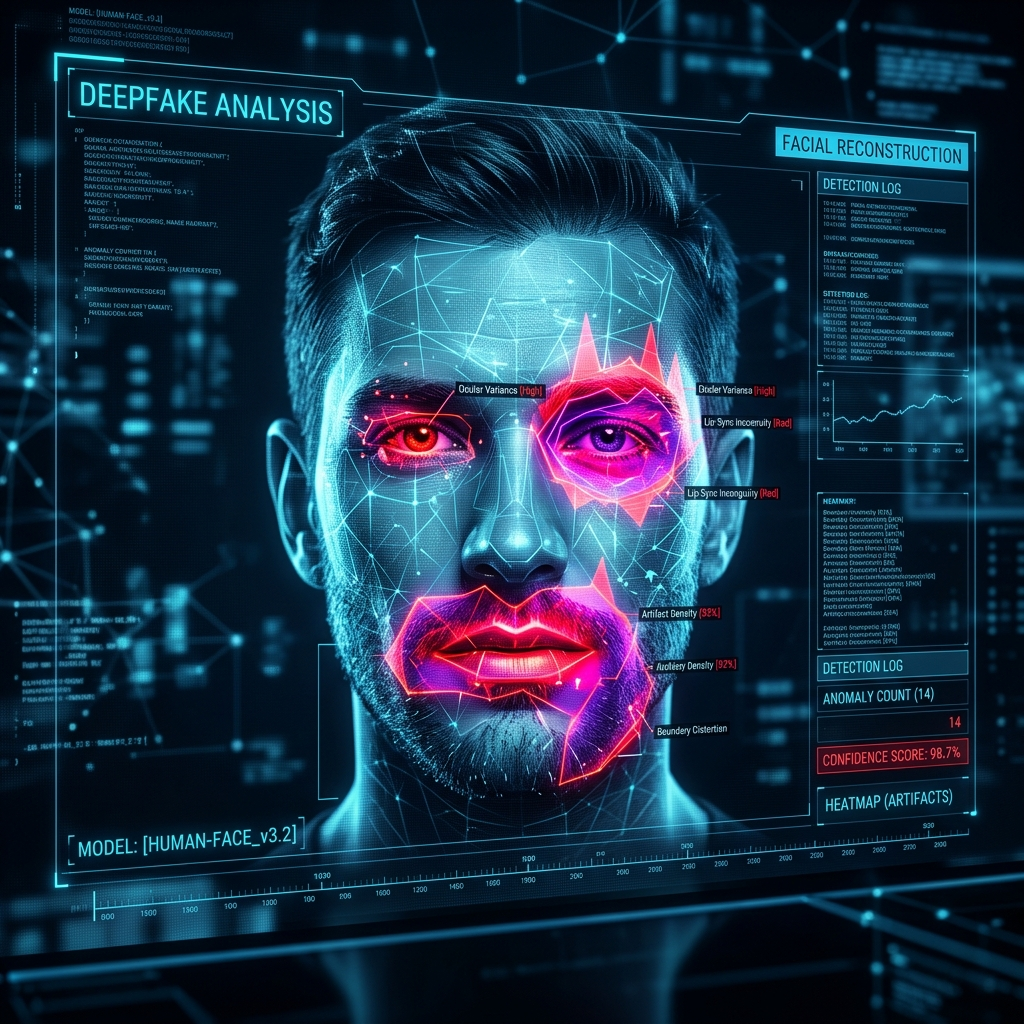
\includegraphics[width=0.9\linewidth]{heatmap.jpg}
    \end{center}
    \vspace{0.5cm}
\end{block}
\end{column}

% ==================== COLUMN 3 ====================
\begin{column}{.31\paperwidth}
\begin{block}{Attention-Based Artifact Detection}
    \vspace{1cm}
    \begin{center}
        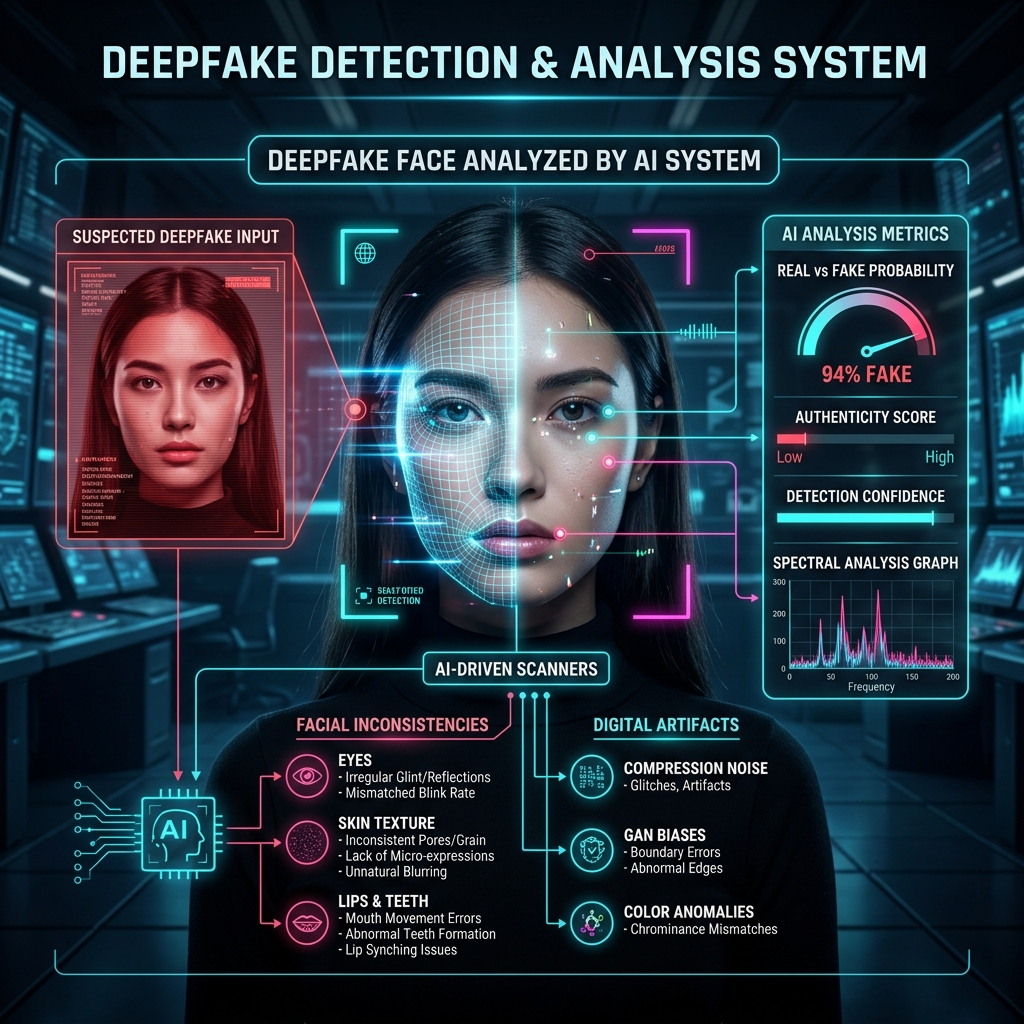
\includegraphics[width=0.9\linewidth]{sleek_concept.jpg}
    \end{center}
    \vspace{1cm}
    \centering \Large \textit{Unlike macroscopic facial analysis, our Transformer-based model targets subtle spatial-temporal inconsistencies and boundary warping where generators fail.}
    \vspace{1cm}
\end{block}

\begin{block}{Impact \& Future Scope}
    \vspace{0.5cm}
    \begin{center}
    \resizebox{0.9\linewidth}{!}{
        \begin{tikzpicture}[node distance=1.5cm and 0cm]
            \node (trust) [rectangle, draw=neoncyan, fill=bgblock, text=white, very thick, minimum width=15cm, minimum height=3cm, align=center, drop shadow] {\Huge \textbf{Restoring Digital Trust} \\ \Large Empowering journalists to verify media authenticity.};
            
            \node (future) [rectangle, draw=neonmagenta, fill=bgblock, text=white, very thick, minimum width=15cm, minimum height=3cm, align=center, drop shadow, below=1cm of trust] {\Huge \textbf{The Road Ahead} \\ \Large Expanding to Multimodal Audio/Visual Detection.};
            
            \draw [arrow, neoncyan] (trust) -- (future);
        \end{tikzpicture}
    }
    \end{center}
    \vspace{0.5cm}
\end{block}
\end{column}

\end{columns}
\end{frame}
\end{document}
